%-----------------------------------------------------------------------------%
\chapter{\babEmpat}
%-----------------------------------------------------------------------------%

\section{Definisi Lingkup}

\subsection{Pernyataan Masalah, Peluang dan Arahan}

Sebagaimana dipaparkan pada bab Pendahuluan, UMS telah memiliki sistem SSO dengan data \f{\gls{credential}} tersimpan dalam \GLS{ldap} dan dikelola dengan sebuah aplikasi tersendiri. Masalah yang muncul adalah bahwa data \GLS{ldap} sering tidak sinkron dengan data Sistem Informasi Kepegawaian dan Sistem Informasi Kemahasiswaan sebagai sumbernya. Di samping itu, terjadi dobel pekerjaan ketika menambah, mengubah dan menghapus data ke \GLS{ldap} dan server surel (\textit{Goole Apps}). 

\subsection{Pernyataan Tentang Solusi yang Diharapkan}
Aplikasi yang diusulkan memberikan lapisan antara yang menghubungan Sistem Informasi Kepegawaian dan Sistem Informasi Kemahasiswaan dengan \GLS{ldap} dan menghubungkan \GLS{ldap} dengan \textit{Google Apps}.

\begin{table}[ht]
  \centering
  \caption{Pernyataan Masalah dan Solusi}
  \renewcommand{\arraystretch}{1.5}% Spread rows out...
  \begin{tabular}
  {|>{}m{6.2cm}| 
    >{\centering}m{4cm}| 
    >{\centering\arraybackslash}m{2.50cm}|}
    \hline\hline
    \bo{Masalah, Peluang dan Arahan} & 
    \bo{Solusi yang Diajukan} & 
    \bo{Urutan Prioritas}\\
    \hline
    Data \GLS{ldap} sering tidak sinkron dengan data Sistem Informasi Kepegawaian dan Sistem Informasi Kemahasiswaan sebagai sumbernya.  & 
    Pengembangan aplikasi baru & 1 \\

   Terjadi dobel pekerjaan ketika menambah, mengubah dan menghapus data ke \GLS{ldap} dan server surel (\textit{Goole Apps}).  & 
    Pengembangan aplikasi baru & 2 \\

    \hline
  \end{tabular}
\end{table}


\newpage
\section{Analisis Masalah}

\begin{table}[ht]
\caption{Masalah, Peluang, Tujuan dan Pembatas}
\begin{tabular}{|p{3.75cm}|p{3cm}|p{3.50cm}|p{2cm}|}
\hline
\multicolumn{2}{|c|}{\bo{Analisis Sebab Akibat}} &
\multicolumn{2}{c|}{\bo{Tujuan Perbaikan Sistem}}\\
\hline
\centering \bo{Masalah/Peluang} & 
\centering \bo{Sebab Akibat} &
\centering \bo{Tujuan Sistem} &
\multicolumn{1}{c|}{\bo{Pembatas}}\\
\hline
\centering Data \GLS{ldap} sering tidak sinkron dengan data Sistem Informasi Kepegawaian dan Sistem Informasi Kemahasiswaan sebagai sumbernya. &
\centering Terjadi duplikasi data dan data \GLS{ldap} tidak tervalidasi. &
\centering Dibuat aplikasi web service yang memungkinkan untuk menghidari duplikasi data dan memvalidasinya. & 
{Aplikasi harus aman.}\\
\hline
\centering Terjadi dobel pekerjaan ketika menambah, mengubah dan menghapus data ke \GLS{ldap} dan server surel (\textit{Goole Apps}). &
\centering Pekerjaan tidak efisien. &
\centering Dibuat aplikasi web service yang memungkinkan sinkronisasi \GLS{ldap} dengan \textit{Google Apps} secara otomatis. &
{Aplikasi harus aman.} \\
\hline
\end{tabular}
\end{table}

\newpage
\section{Analisis Kebutuhan}

\begin{table}[ht]
  \caption{Daftar Kebutuhan}
  \renewcommand{\arraystretch}{1.5}% Spread rows out...
  \begin{tabular}
  {|>{}m{10.75cm}| 
    >{\centering\arraybackslash}m{2.5cm}|}
    \hline\hline
    \bo{Kebutuhan} & 
    \bo{Klasifikasi}\\
    \hline
    Sistem harus mengijinkan aplikasi ter-authentikasi menelusur data pengguna. &
    Fungsional\\
    \hline
    Sistem harus mengijinkan aplikasi ter-authentikasi menambah, mengubah dan menghapus data pengguna. &
    Fungsional\\
    \hline
    Sistem harus mengijinkan aplikasi ter-authentikasi menambah, mengubah dan menghapus data \gls{surel} pengguna. &
    Fungsional\\
    \hline
    Sistem harus mengijinkan aplikasi ter-authentikasi melakukan sinkronisasi data pengguna ke \textit{Google Apps}. &
    Fungsional\\
    \hline
    Sistem harus mengijinkan aplikasi ter-authentikasi mengubah password \textit{Google Apps}. &
    Fungsional\\
    \hline
    Sistem harus mengijinkan aplikasi ter-authentikasi menampilkan \gls{surel} alias pengguna \textit{Google Apps}. &
    Fungsional\\
    \hline
    Sistem harus mengijinkan aplikasi ter-authentikasi menampilkan dan mengubah alamat pengiriman \gls{surel} pengguna \textit{Google Apps}. &
    Fungsional\\
    \hline
    Sistem harus mengijinkan aplikasi ter-authentikasi mendelegasikan akun \gls{surel} pengguna \textit{Google Apps}. &
    Fungsional\\
    \hline
    Sistem yang dibangun adalah \textit{web service} menggunakan bahasa pemrograman Python&
    Non fungsional\\
    \hline
  \end{tabular}
\end{table}

\newpage
\section{Desain Logis}

\subsection{Use-case}

\singlespacing
\begin{table}[H]
\caption{Daftar \textit{Use-case}}
\renewcommand{\arraystretch}{1.5}% Spread rows out...
\begin{tabular}
{|>{\centering}m{4cm}|
   >{\centering}m{7.25cm}| 
   >{\centering\arraybackslash}m{2cm}|}
\hline\hline
\bo{Nama Use-case} & \bo{Deskripsi Use-case} & \bo{Aktor}\\
\hline
Menelusur Data Pengguna &
Use-case yang mendeskripsikan proses penelusuran data \GLS{ldap} &
\acrshort{api} Client\\
\hline
Menambah, Mengubah dan Menghapus Data Pengguna &
Use Case yang mendeskripsikan proses menambah, mengubah dan menghapus data pengguna di \GLS{ldap} &
\acrshort{api} Client\\
\hline
Menampilkan, Menambah dan Menghapus Email Pengguna &
Use Case yang mendeskripsikan proses menampilkan, menambah dan menghapus \gls{surel} pengguna di \GLS{ldap} &
\acrshort{api} Client\\
\hline
Menampilkan, Menambah dan Menghapus Jabatan Pengguna &
Use Case yang mendeskripsikan proses menampilkan, menambah dan menghapus jabatan pengguna di \GLS{ldap} &
\acrshort{api} Client\\
\hline
Sinkronisasi Data ke \textit{Google Apps} &
Use Case yang mendeskripsikan proses sinkronisasi data ke \textit{Google Apps} &
\acrshort{api} Client\\
\hline
Mengubah Password \textit{Google Apps} &
Use Case yang mendeskripsikan proses mengubah password pengguna di \textit{Google Apps} &
\acrshort{api} Client\\
\hline
Menampilkan Alias Email \textit{Google Apps} &
Use Case yang mendeskripsikan proses menampilkan alias \gls{surel} pengguna di \textit{Google Apps} &
\acrshort{api} Client\\
\hline
Menampilkan dan Menambah Alamat Pengiriman Email \textit{Google Apps} &
Use Case yang mendeskripsikan proses menampilkan dan menambah alamat pengiriman \gls{surel} pengguna di \textit{Google Apps} &
\acrshort{api} Client\\
\hline
Mengelola Delegasi Email \textit{Google Apps}&
Use Case yang mendeskripsikan proses pendelegasian \gls{surel} pengguna di \textit{Google Apps} &
\acrshort{api} Client\\
\hline
\end{tabular}
\end{table}
\doublespacing

\subsection{Daftar Entitas}

\textbf{Atribut LDAP yang digunakan} \cite{biondo2001}:\\
uid: user id unik/nama login\\
givenName: nama depan\\
sn: nama belakang\\
cn: nama lengkap\\
userPassword: password\\
postalAddress: alamat\\
l: kota\\
st: propinsi\\
postalCode: kode pos\\
mail: alamat surel\\
telephoneNumber: telpon rumah\\
mobile: nomor hp\\
employeeNumber: NIK/NIP\\
employeeType: jenis karyawan/mahasiswa\\
departmentNumber: nomor unit/fakultas\\
ou: nama unit/fakultas\\

\subsection{Model Proses}

\begin{figure}
	\centering
	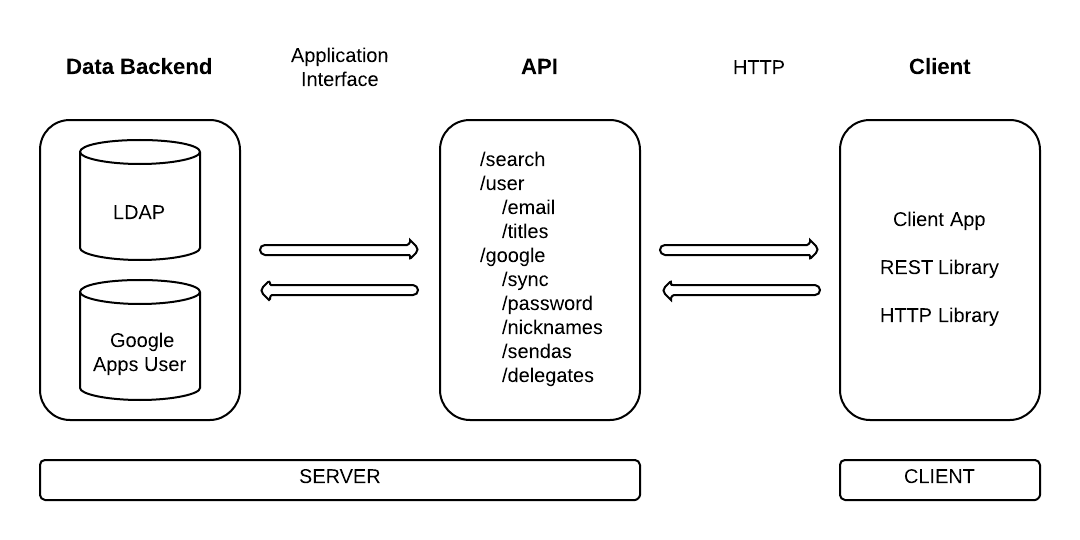
\includegraphics[width=1\textwidth]
		{pics/processmodel.png}
	\caption{Model Proses}
	\label{fig:model}
\end{figure}

\section{Desain Fisik}

Aplikasi yang dibangun menggunakan authentikasi \textit{Basic Authentication} yang merupakan kombinasi \textit{username} dan \textit{password}. \textit{Request} dan \textit{Response} hanya menggunakan format \textit{JSON}.

\subsection{Menelusur Data Pengguna}

POST https://accounts.ums.ac.id/search

\noindent
\textit{JSON Request:}
\begin{lstlisting}
{
    "filter": "uid=ya931"
}
\end{lstlisting}

\noindent
\textit{JSON Response:}
\begin{lstlisting}
[
    [
        "uid=ya931,ou=Employee,ou=People,dc=ums,dc=ac,dc=id",
        {
            "uid": ["ya931"],
            "givenName": ["Suyadi"],
            "sn": ["Abufarros"],
            "cn": ["Suyadi Abufarros"],
            "postalAddress": ["Purbayan Baki"],
            "l": ["Sukoharjo"],
            "st": ["Jateng"],
            "c": ["Indonesia"],
            "postalCode": ["57102"],
            "mail": ["suyadi@ums.ac.id", "abufarros@gmail.com"],
            "telephoneNumber": ["0271222222"],
            "mobile": ["081234556"],
            "employeeNumber": ["931"],
            "employeeType": ["Karyawan Tetap"],
            "departmentNumber": ["345"],
            "ou": [ "UIT"],
            "title": ["STAF"]
        }
    ],
]
\end{lstlisting}

\subsection{Menambah Data Pengguna}

POST https://accounts.ums.ac.id/users

\noindent
\textit{JSON Request:}
\begin{lstlisting}
{
    "userType": "EMPLOYEE",
    "uniID": "abc123",
    "firstName": "Muhammad",
    "lastName": "Surono",
    "userPassword": "qwerty",
    "postalAddress": "Pabelan",
    "city": "Solo",
    "state": "Jateng",
    "postalCode": "57102",
    "mail": "abc123@gmail.com",
    "telephoneNumber": "0271222222",
    "mobile": "081234556",
    "employeeNumber": "876",
    "employeeType": "Dosen",
    "departmentNumber": "345",
    "ou": "Teknik Informatika"
}
\end{lstlisting}

\noindent
\textit{Text Response:}\\
- \textbf{Ok}: berhasil menambahkan data\\
-  \textbf{Not ok}: gagal menambahkan data

\subsection{Mengubah Data Pengguna}

PUT https://accounts.ums.ac.id/users

\noindent
\textit{JSON Request:}
\begin{lstlisting}
{
    "userType": "EMPLOYEE",
    "uniID": "abc123",
    "firstName": "Muhammad",
    "lastName": "Surono",
    "userPassword": "qwerty",
    "postalAddress": "Pabelan",
    "city": "Solo",
    "state": "Jateng",
    "postalCode": "57102",
    "mail": "abc123@gmail.com",
    "telephoneNumber": "0271222222",
    "mobile": "081234556",
    "employeeNumber": "876",
    "employeeType": "Dosen",
    "departmentNumber": "345",
    "ou": "Teknik Informatika"
}
\end{lstlisting}

\noindent
\textit{Text Response:}\\
- \textbf{Ok}: berhasil menambahkan data\\
-  \textbf{Not ok}: gagal menambahkan data

\subsection{Menghapus Data Pengguna}

DELETE https://accounts.ums.ac.id/users

\noindent
\textit{JSON Request:}
\begin{lstlisting}
{
    "uniID": "abc123"
}
\end{lstlisting}

\noindent
\textit{Text Response:}\\
- \textbf{Ok}: berhasil menambahkan data\\
-  \textbf{Not ok}: gagal menambahkan data


\subsection{Menampilkan Email Pengguna}

POST https://accounts.ums.ac.id/user/email

\noindent
\textit{JSON Request:}
\begin{lstlisting}
{
    "uniID": "ya931"
}
\end{lstlisting}

\noindent
\textit{JSON Response:}
\begin{lstlisting}
[
    "Suyadi@ums.ac.id",
    "Suyadi.Abufarros@ums.ac.id"
]
\end{lstlisting}

\subsection{Menambah Email Pengguna}

PUT https://accounts.ums.ac.id/user/email

\noindent
\textit{JSON Request:}
\begin{lstlisting}
{
    "uniID": "ya931",
    "email": "suyadi@ums.ac.id"
}
\end{lstlisting}

\noindent
\textit{Text Response:}\\
- \textbf{Ok}: berhasil menambahkan data\\
-  \textbf{Not ok}: gagal menambahkan data

\subsection{Menghapus Email Pengguna}

DELETE https://accounts.ums.ac.id/user/email

\noindent
\textit{JSON Request:}
\begin{lstlisting}
{
    "uniID": "ya931",
    "email": "suyadi@ums.ac.id"
}
\end{lstlisting}

\noindent
\textit{Text Response:}\\
- \textbf{Ok}: berhasil menambahkan data\\
-  \textbf{Not ok}: gagal menambahkan data

\subsection{Menampilkan Jabatan Pengguna}

POST https://accounts.ums.ac.id/user/titles

\noindent
\textit{JSON Request:}
\begin{lstlisting}
{
    "uniID": "ya931"
}
\end{lstlisting}

\noindent
\textit{JSON Response:}
\begin{lstlisting}
[
    "CNF",
    "Admin"
]
\end{lstlisting}

\subsection{Menambah Jabatan Pengguna}

PUT https://accounts.ums.ac.id/user/titles

\noindent
\textit{JSON Request:}
\begin{lstlisting}
{
    "uniID": "ya931",
    "title": "Admin"
}
\end{lstlisting}

\noindent
\textit{Text Response:}\\
- \textbf{Ok}: berhasil menambahkan data\\
-  \textbf{Not ok}: gagal menambahkan data

\subsection{Menghapus Jabatan Pengguna}

DELETE https://accounts.ums.ac.id/user/titles

\noindent
\textit{JSON Request:}
\begin{lstlisting}
{
    "uniID": "ya931",
    "title": "Admin"
}
\end{lstlisting}

\noindent
\textit{Text Response:}\\
- \textbf{Ok}: berhasil menambahkan data\\
-  \textbf{Not ok}: gagal menambahkan data

\subsection{Sinkronisasi Data ke \textit{Google Apps}}

POST https://accounts.ums.ac.id/google/sync

\noindent
\textit{JSON Request:}
\begin{lstlisting}
{
    "uniID": "ya931"
}
\end{lstlisting}

\noindent
\textit{Text Response:}\\
- \textbf{Ok}: berhasil menambahkan data\\
-  \textbf{Not ok}: gagal menambahkan data

\subsection{Mengubah Password \textit{Google Apps}}

POST https://accounts.ums.ac.id/google/password

\noindent
\textit{JSON Request:}
\begin{lstlisting}
{
    "uniID": "ya931",
    "password": "mypassword"
}
\end{lstlisting}

\noindent
\textit{Text Response:}\\
- \textbf{Ok}: berhasil menambahkan data\\
-  \textbf{Not ok}: gagal menambahkan data

\subsection{Menampilkan Alias Email \textit{Google Apps}}

POST https://accounts.ums.ac.id/google/nicknames

\noindent
\textit{JSON Request:}
\begin{lstlisting}
{
    "uniID": "ya931"
}
\end{lstlisting}

\noindent
\textit{JSON Response:}
\begin{lstlisting}
[
    "suyadi",
    "suyadi.abufarros"
]
\end{lstlisting}

\subsection{Menampilkan Alamat Pengiriman Email \textit{Google Apps}}

POST https://accounts.ums.ac.id/google/sendas

\noindent
\textit{JSON Request:}
\begin{lstlisting}
{
    "uniID": "ya931",
}
\end{lstlisting}

\noindent
\textit{JSON Response:}
\begin{lstlisting}
[
    "suyadi@ums.ac.id",
    "suyadi.abufarros@ums.ac.id"
]
\end{lstlisting}

\subsection{Menambah Alamat Pengiriman Email \textit{Google Apps}}

PUT https://accounts.ums.ac.id/google/sendas

\noindent
\textit{JSON Request:}
\begin{lstlisting}
{
    "uniID": "ya931",
    "address": "suyadi@ums.ac.id"
}
\end{lstlisting}

\noindent
\textit{Text Response:}\\
- \textbf{Ok}: berhasil menambahkan data\\
-  \textbf{Not ok}: gagal menambahkan data

\subsection{Menampilkan Delegasi Email \textit{Google Apps}}

POST https://accounts.ums.ac.id/google/delegates

\noindent
\textit{JSON Request:}
\begin{lstlisting}
{
    "uniID": "ithelpdesk"
}
\end{lstlisting}

\noindent
\textit{JSON Response:}
\begin{lstlisting}
[
    "ya123@ums.ac.id",
    "wd123@ums.ac.id"
]
\end{lstlisting}

\subsection{Menambah Delegasi Email \textit{Google Apps}}

PUT https://accounts.ums.ac.id/google/delegates

\noindent
\textit{JSON Request:}
\begin{lstlisting}
{
    "uniID": "ithelpdesk",
    "nickname": "ya123@ums.ac.id"
}
\end{lstlisting}

\noindent
\textit{Text Response:}\\
- \textbf{Ok}: berhasil menambahkan data\\
-  \textbf{Not ok}: gagal menambahkan data

\subsection{Menghapus Delegasi Email \textit{Google Apps}}

DELETE https://accounts.ums.ac.id/google/nicknames

\noindent
\textit{JSON Request:}
\begin{lstlisting}
{
    "uniID": "ithelpdesk",
    "nickname": "ya123@ums.ac.id"
}
\end{lstlisting}

\noindent
\textit{Text Response:}\\
- \textbf{Ok}: berhasil menambahkan data\\
-  \textbf{Not ok}: gagal menambahkan data

\section{Konstruksi dan Testing}

Penulis menggunakan \textit{Flask Framework} dalam mengembangkan aplikasi ini. \textit{Flask} adalah sebuah \textit{framework} mikro untuk mengembangkan aplikasi web berbahasa \textit{Python}. "Mikro" bukan berarti aplikasi web yang dibuat hanya terdiri dari sebuah file, walaupun memungkinkan, juga bukan berarti memiliki fungsionalitas terbatas, tetapi lebih ditekankan pada kesedarhanaan  dan \textit{extensible}.

Untuk mengembangkan aplikasi berbasis \textit{Flask} tidak memerlukan spesifikasi perangkat yang tinggi, tetapi butuh koneksi internet, karena data \textit{Google Apps} tersimpan di server \textit{Google}. Secara rinci, kebutuhan pengembangan aplikasi ini sebagai berikut:

\begin{enumerate}[itemsep=-1ex]
\item Laptop dengan sistem operasi Windows, Linux atau sistem operasi lain yang kompatibel dengan \textit{Python}.
\item Bahasa pemrograman \textit{Python} dan \textit{Python Setuptools}.
\item Beberapa paket \textit{Python} yang dibutuhkan: \textit{Flask, Python-LDAP, Gdata, dll.}
\end{enumerate}

%\lstinputlisting[language=Python]{code/simple-client/simple.py}

\section{Instalasi}

Ada beberapa cara untuk menginstall aplikasi ke server produksi yang salah satunya menggunakan \textit{Gunicorn} dan \textit{Nginx} pada \textit{Linux Debian}. \textit{Gunicorn (Green Unicorn)} adalah \textit{Web Server Gateway Interface (WSGI)}. \textit{Nginx} adalah web server yang difungsikan sebagai \textit{proxy}. Menurut Benoit Chesneau, sangat direkomendasikan \textit{Gunicorn} digunakan bersama \textit{proxy} server \cite{benoit2012}.